\chapter{Août 2022}

\paragraph{Question 1.} \textit{Oscillateur Harmonique.}\\

En unités sans dimensions ($\hbar=1$), les opérateurs position $\hat x$ et impulsion $\hat p$ obéissent à la relation de commutation canonique $[\hat x, \hat p]=i $.  Nous noterons $\lvert x \rangle$ et $\lvert p \rangle$ les états propres de $\hat x$ et de $\hat p $ respectivement, pour tout $x, p \in \mathbb{R}$.

Les opérateurs de création et destruction sont définis par 
$\hat a= \frac{1}{\sqrt{2}}(\hat x+i\hat p)$, $a^\dagger= \frac{1}{\sqrt{2}}(\hat x-i\hat p)$ et satisfont donc $[\hat a,\hat a^\dagger]=1$. L'opérateur nombre $\hat n$ est donné par $\hat n= \hat a^\dagger \hat a$ et ses vecteurs propres sont notés $\hat n \ket{n} =n \ket{n}$ où $n \in \mathbb{N}$. 

L'hamiltonien de l'oscillateur harmonique est $\hat H = \frac{1}{2}\omega ( \hat P^2 + \hat X^2 ) = \omega (\hat n + 1/2)\ $. \\

Soit l'état $\vert \psi \rangle$ qui dans la base nombre s'écrit
\begin{equation}
\vert \psi \rangle = \alpha \vert n \rangle + \beta \vert n+1 \rangle 
\end{equation}
avec $n\geq 0$ un entier, et $\alpha,\beta \in \mathbb{C}$ deux nombres complexes satisfaisant $\vert \alpha \vert^2 + \vert \beta \vert^2=1$.

\begin{enumerate}
\item 
Donnez la forme des états $a \vert \psi \rangle$ et $a^\dagger \vert \psi \rangle$ (dans la base nombre).
\item
Que valent les valeurs moyennes\\
de $\hat x$, \\
de $\hat p$, \\
de $\hat x^2$\\
dans l'état $\vert \psi \rangle$ ?

\end{enumerate}
Donnez les réponses 
en fonction de $\alpha, \beta, n$. N'oubliez pas que $\alpha$ et $\beta$ sont complexes.

\paragraph{Question 2.} \textit{Photon se propageant dans un millieu optiquement actif.} \\






Le nombre d'onde $k$ d'un photon de fréquence angulaire $\omega$ se propageant dans un milieu d'indice de réfraction $n$ est donné par
\begin{equation}
k= \frac{n \omega}{c} 
\end{equation}
avec $c$ la vitesse de la lumière dans le vide.
La fonction d'onde d'un tel photon se propageant dans la direction des z positifs est donnée par
\begin{equation}
\psi(t,z) = A e^{-i \omega t} e^{i k z}\ .
\end{equation}


La polarisation d'un photon est décrit par un espace de Hilbert ${\cal H}_{pol}$ de dimension 2.

Nous noterons $\vert V\rangle$ et $\vert H\rangle$ les états correspondant à un photon polarisé verticalement et horizontalement. Ces deux états constituent une base orthonormée de l'espace de Hilbert ${\cal H}_{pol}$ .

Un photon dans un état de polarisation linéaire, à un angle $\theta$ de la verticale ($\theta \in [0,\pi/2[$) est dans l'état 
\begin{equation}
\vert \theta \rangle = \cos \theta \vert V\rangle + \sin \theta \vert H\rangle\ .
\label{eq:theta}
\end{equation}

Un polariseur orienté selon l'axe $\theta$ laissera passer la lumière dans l'état 
$\vert \theta \rangle$ et absorbera la lumière dans l'état $\vert \theta + \pi/2 \rangle$. Il peut donc être vu comme un système de mesure quantique qui mesure dans la base $\vert \theta \rangle$ et $\vert \theta +\pi/2 \rangle$


Nous pouvons également utiliser la base de polarisation circulaire droite et gauche donnée par 
\begin{eqnarray}
\vert D \rangle &=& \frac{1}{\sqrt{2}} \vert V\rangle + \frac{i}{\sqrt{2}} \vert H\rangle\nonumber\\
\vert G \rangle &=& \frac{1}{\sqrt{2}} \vert V\rangle - \frac{i}{\sqrt{2}} \vert H\rangle\ .
\end{eqnarray}



Certaines molécules sont chirales: il existe deux formes distinctes (appelés énantiomères) de la molécule qui sont image miroir l'une de l'autre. De nombreuses molécules organiques (par exemple des sucres, des acides animés) sont des molécules chirales. Généralement les être vivants utilisent un seul des énantiomères, mais pas l'autre. Par exemple l'isomère D du glucose, appelé dextrose, est très répandu dans le milieu naturel, mais pas l'isomère L.

Si un liquide (par exemple de l'eau) contient en solution une plus grande quantité d'un énantiomère d'une molécule chirale, il devient optiquement actif. Par exemple de l'eau avec du dextrose dissout est optiquement actif.

Dans un milieu optiquement actif, lles polarisations gauche et droite percoivent des indices de réfraction différents, notés $n_G$ et $n_D$.
La fonction d'onde d'un photon de polarisation gauche ou droite est donc donnée par
\begin{eqnarray}
\vert \psi_G(t,z)\rangle  = \exp \left( -i \omega t + i \frac{n_G \omega}{c} z\right) \vert G\rangle  \ , \nonumber\\
 \vert  \psi_D(t,z)  \rangle =  \exp \left(  -i \omega t + i \frac{n_D \omega}{c} z \right) \vert D\rangle \  .
 \label{eq:psiGD}
\end{eqnarray}




\begin{figure}
\centering
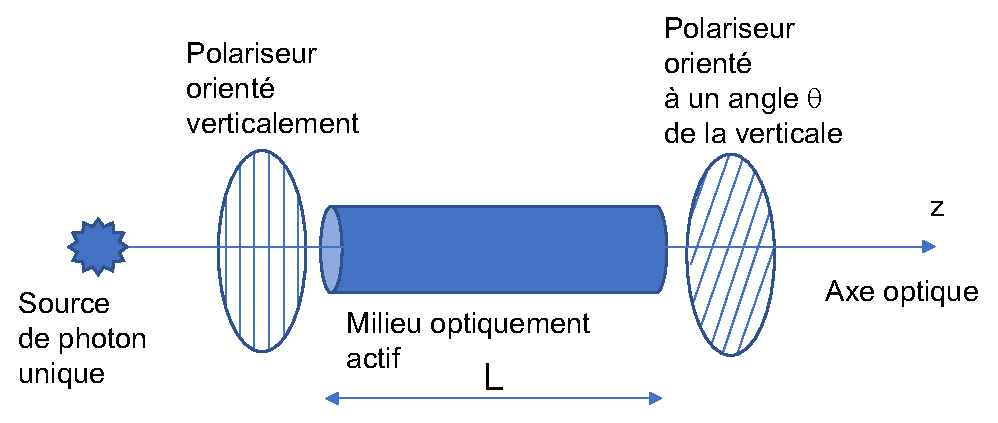
\includegraphics[scale=0.8]{Pictures/Fig-Pol.pdf}
\end{figure}

Nous considérons le dispositif illustré dans la figure consititué d'une source de photon unique, d'un polariseur, d'un tube de longueur $L$ contenant un liquide optiquement actif. Le tube est suivi d'un second polariseur dont on peut faire tourner l'orientation pour analyser la polarisation après passage dans le liquide.

Si le photon traverse le premier polariseur il est dans l'état $\vert V \rangle$.

Montrer qu'à la sortie du tube contenant le liquide optiquement actif, le photon est dans un état de polarisation linéaire selon la direction $\theta = \frac{(n_G - n_D) \omega L}{2 c}$.
(Pour cela nous recommandons d'exprimer l'état $\vert V \rangle$ à la sortie du polariseur dans la base $\vert G\rangle, \vert D \rangle$; d'utiliser l'équation \eqref{eq:psiGD} pour obtenir l'état à la sortie du liquide; de repasser dans la base $\vert H\rangle, \vert V \rangle$; et puis de comparer l'état ainsi obtenu avec l'équation \eqref{eq:theta}).





\paragraph{Question 3.} \textit{Etat propre de l'Hamiltonien d'énergie nulle.} \\

\begin{figure}
\centering
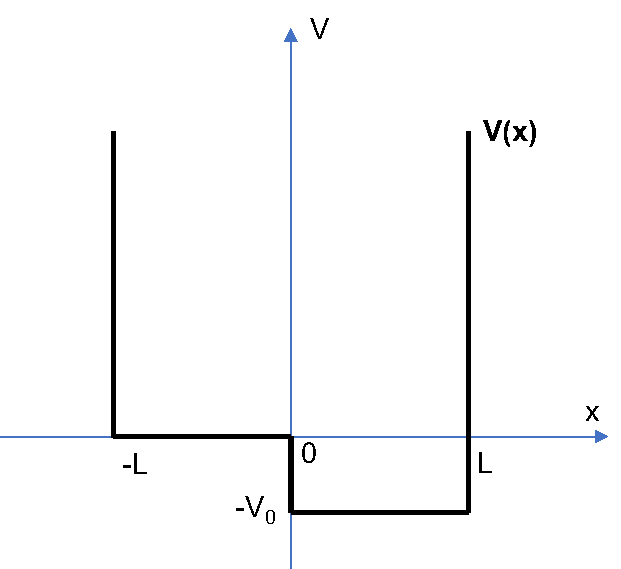
\includegraphics[scale=0.8]{Pictures/FigPot.pdf}
\end{figure}


Considérons une particule de masse $m$ se déplacant dans un potentiel à une dimension $V(x)$. Les états propres de l'hamiltonien satisfont  à l'équation
\begin{equation}
E \psi(x) = - \frac{\hbar^2}{2 m} \partial_x^2 \psi(x) + V(x) \psi(x)
\end{equation}

Le potentiel a
la forme suivante (voir figure):
\begin{eqnarray}
V(x)=+\infty &\quad , \quad& x<-L\nonumber\\
V(x)=0 &\quad , \quad& -L\leq x < 0 \nonumber\\
V(x)=-V_0 &\quad , \quad& 0 \leq x < L \nonumber\\
V(x)=+\infty &\quad , \quad& L\leq x \ .
\end{eqnarray}

Nous supposerons que $L$ est fixé, mais que $V_0>0$ est un paramètre qui peut être ajusté expérimentalement.

Nous cherchons à déterminer les valeurs de $V_0$ telles que l'hamiltonien ait une état propre d'énergie $E=0$.

\newpage

\begin{enumerate}
\item
En supposant $E=0$, écrire les équations auxquelles doit satisfaire $\psi(x)$ dans les différentes régions de l'espace.

\item
Donner les conditions au bord (en $x=-L$ et $x=+L$) et les conditions de raccord là ou le potentiel est discontinu (en $x=0$).

\item
Résoudre ces équations et obtenir une équation implicite pour $V_0$ telle que l'hamiltonien ait un été lié d'énergie $E=0$.
\item

Les deux premières solutions de $$z+ \tan z =0$$ 
(pour $z\geq 0$) sont
$z=0$ et $z=2.03$. Utilisez cette information pour déterminer la  plus petite valeur de $V_0$ telle que l'hamiltonien ait un été lié d'énergie $E=0$.


\end{enumerate}